% -*- LaTeX -*-

% Add proof example to 54
% Resolution: inference rule, proof trees, semantic interpretation,
% rule interpretation, soundness and completeness

\documentclass[handout,x11names,unknownkeysallowed]{beamer}
%\documentclass[x11names]{beamer}
\usepackage{beamerthemeUAB}
\usepackage{verbatim}
\usepackage{color}
\usepackage{multirow}
\usepackage{cite}
%\usepackage{amsthm}
%\setbeamertemplate{theorems}[numbered]
%\newtheorem{proposition}{Proposition}
%\newtheorem{cor}{Corollary}
% -*- LaTeX -*-
%\usepackage{pgfpages}
%\usepackage{handoutWithNotes}
%
%\pgfpagesuselayout{3 on 1 with notes}[a4paper,border shrink=5mm]


\usepackage{subfigure,bm}
\usepackage{multicol}
\usepackage{amsmath}
\usepackage{epsfig}
\usepackage{graphicx}
\usepackage[all,knot]{xy}
\usepackage{marvosym}
\xyoption{arc}
\usepackage{url}
\usepackage{multimedia}
\usepackage{hyperref}
\usepackage[english]{babel}
\usepackage[latin1]{inputenc}
\usepackage{times}
\usepackage{caption}
%\usepackage[T1]{fontenc}
% Or whatever. Note that the encoding and the font should match. If T1
% does not look nice, try deleting the line with the fontenc.
\newcommand{\conv}{\stackrel{\mathbb{D}}{\longrightarrow}}
\newcommand{\cons}{\stackrel{p}{\longrightarrow}}
\newcommand{\nc}{\newpage \clearpage}
\newcommand{\etal}{\textit{et al.}}

\def\boldp{\mathbf p}
\def\btheta{\bm \theta}
\def\bpi{\bm \pi}

\title[] % (Called "`Short Title"', optional, use only with long paper titles)
{Simple Linear Regression}

%\subtitle{EPID 753} % (optional)

\author[Dustin Long, PhD] % (optional, use only with lots of authors)
{Dustin~Long, PhD}


\institute[UAB]
{
  Department of Biostatistics\\
	University of Alabama at Birmingham

}

\def\insertcopyright{$\copyright$ 2019 by Dustin Long}
\def\insertslideinfo{\insertshorttitle}

\subject{}
% This is only inserted into the PDF information catalog. Can be left
% out. 



% This code is not needed since the logo is on every page in the lower left-hand corner
%\pgfdeclareimage[height=0.5cm]{university-logo}{unc-gillings-school-of-public-health-logo.png}
%\logo{\pgfuseimage{university-logo}}


% Delete this, if you do not want the table of contents to pop up at
% the beginning of each subsection:
%\AtBeginSubsection[]
%{
%   \begin{frame}<beamer>
%     \frametitle{Outline}
%     \tableofcontents[currentsection,currentsubsection]
%   \end{frame}
% }


% If you wish to uncover everything in a step-wise fashion, uncomment
% the following command: 

%\beamerdefaultoverlayspecification{<+->}

%\input macros.tex

\date[Week 1]{September 3, 2019}

\newcommand{\beamitem}{\begin{itemize}[<+-|alert@+>]}
%\newcommand{\beamitem}{\begin{itemize}}
%\newcommand{\etal}{\textit{et al.}}

%%%%%%%%%%%%%%%%%%%%%%%%%%%%%%%%%%%%%%%%%%%%%%%%%%%%%%%%%%%%%%%%%%%%%%
\begin{document}

\begin{frame}
  \titlepage
\end{frame}

\begin{frame}
Outline:
\begin{itemize}
\item Simple Linear Regression
\end{itemize}

\end{frame}


\begin{frame}
Outline:
\begin{itemize}
\item Assumptions and properties of regression with one variable
\item Determination and measures for the line of best fit 
\item Inference and Interpretations of parameters
\end{itemize}

\end{frame}


%%%%%%%%%%%%%%%%%%%%%%%%%%%%%%%%%%%%%%%%%%%%%%%%%%%%%%%%%%%%%%%%%%%%%%
\section{Assumptions and Properties}
\begin{frame}
\beamitem
\item When do we use linear regression?
\item What type of model do we use?
\item What is the best fitting model, and what do we mean by ``best fit''?
\end{itemize}
\end{frame}

\begin{frame}
\centering
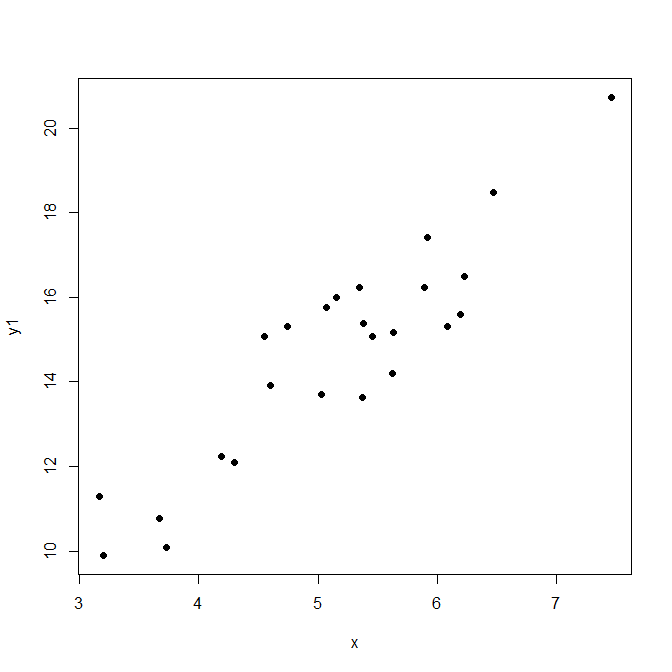
\includegraphics[width=0.48\textwidth]{linear.png}
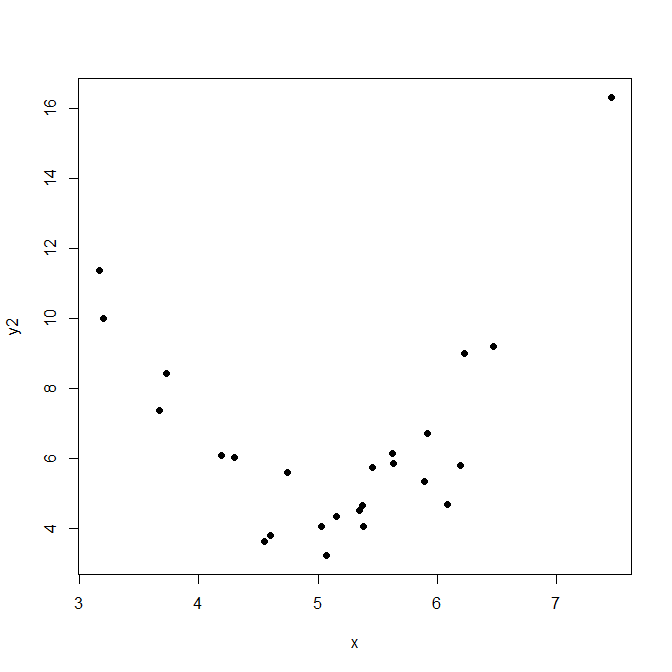
\includegraphics[width=0.48\textwidth]{parabolic.png}
\end{frame}

\begin{frame}

{ \begin{center} 
Example: SBP and Age
\end{center}}
\vspace{.1in}
\begin{center}
\begin{tabular}{ccc}
Obs	&Age	&SBP\\
\hline	
1	&19	&122	\\
2	&25	&125	\\
3	&30	&126	\\
4	&42	&129	\\
5	&46	&130	\\
6	&52	&135	\\
7	&57	&138	\\
8	&62	&142	\\
9	&70	&145\\
\end{tabular}
\end{center}
\end{frame}

\begin{frame}
 \begin{center} 


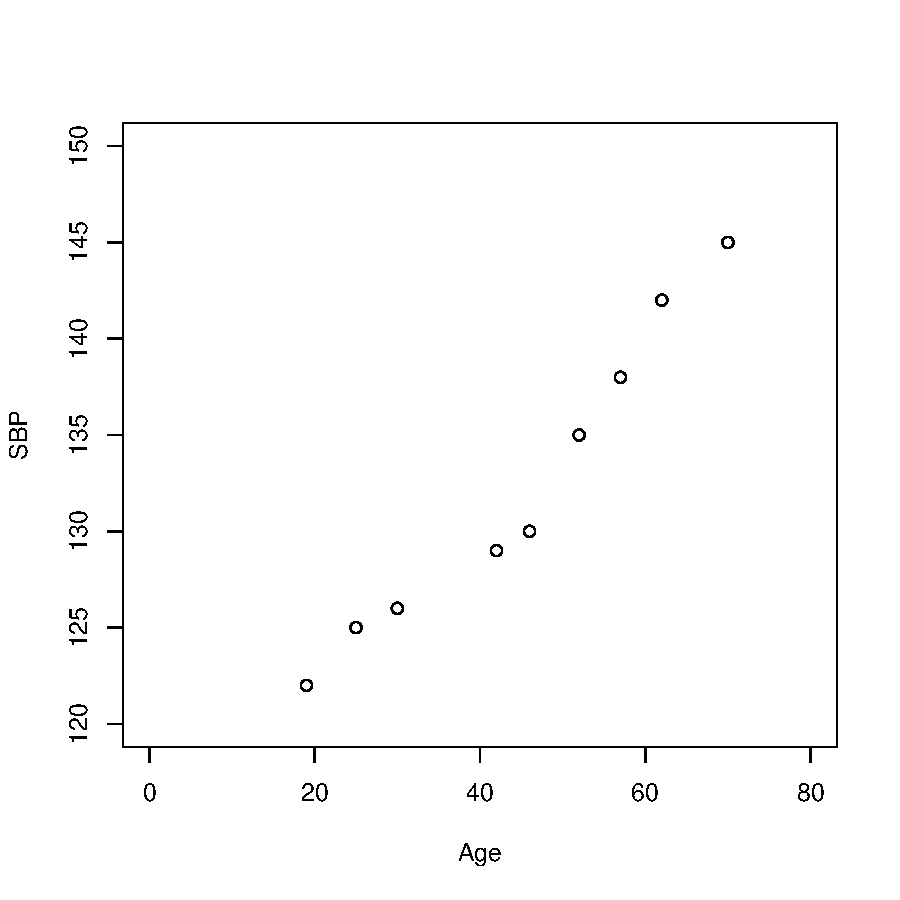
\includegraphics[width=.6\textwidth]{regression_fictitious.pdf}
\end{center}
\end{frame}



\begin{frame}
Mathematical Properties of a Straight Line 

\beamitem
\item A line is defined by an intercept and slope, i.e., $y = Mx + B$
\item Recall properties of straight lines

\end{itemize}
\end{frame}

\begin{frame}
 \begin{center} 



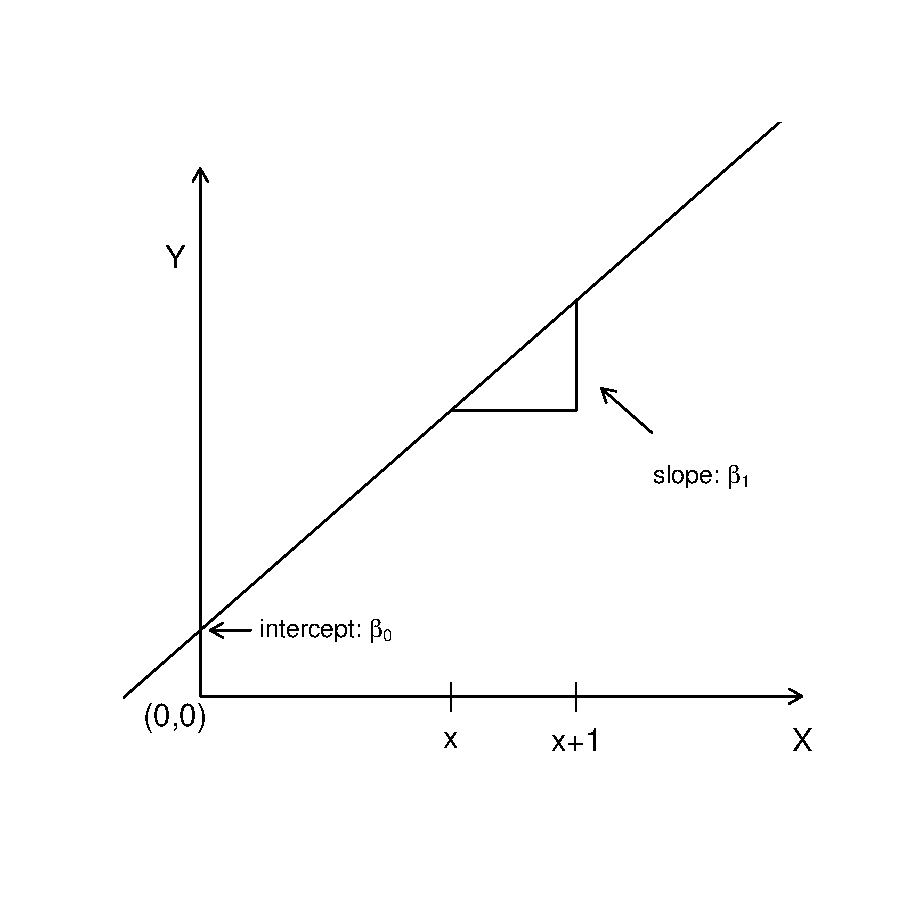
\includegraphics[width=.6\textwidth]{reg_fig2.pdf}
\end{center}
\end{frame}

\begin{frame}
Definition of Linear Regression
\beamitem
\item The model used for simple linear regression is:
\item $Y_i = \beta_0 + \beta_1 X_i + \epsilon_i$
\item where $Y_i$ is a dependent (outcome) random variable, $X_i$ is an independent random variable,  $i=1\ldots n$, $\beta_0$ is the population intercept, $\beta_1$ is the population slope, and $\epsilon_i \sim N(0,\sigma^2)$
\item $\bm{Y} = \bm{X\beta} + \bm{e}$
\end{itemize}
\end{frame}

\begin{frame}
Statistical Assumptions of a Straight Line 

\beamitem
\item Assumption 1: Homoscedasticity, $\sigma_x^2=\sigma^2~~\forall x$
\item Assumption 2: Independence, $Y$ values are independent of one another
\item Assumption 3: Linearity, $E[Y|X=x] = \mu_{Y|X=x} = \beta_0 + \beta_1 x$ or $Y = \beta_0 + \beta_1 x + E$
\item Assumption 4: Existence, ($Y|X=x \sim f(\mu, \sigma_x^2)$, where $\mu,\sigma_x^2 < \infty, ~ \forall x$
\item Assumption 5: Normality, $Y|X=x \sim N(\mu_{Y|X=x},\sigma^2)$

\item 
\end{itemize}
\end{frame}

\begin{frame}
Determining the Best-fitting Line

\beamitem
\item Least Squares Method, OLS \href{http://www.rossmanchance.com/applets/Reg/index.html}{Example}
\item Another \href{http://hspm.sph.sc.edu/COURSES/J716/demos/LeastSquares/LeastSquaresDemo.html}{example}
\item Minimum-variance method, Best Linear Unbiased Estimators (BLUE) 
\item Under Assumptions 1-5, OLS estimates and BLUE are the same
\item $\hat\beta_0 = \bar{Y} - \hat\beta_1\bar{x}$
\item $\hat\beta_1 = \frac{\sum_{i=1}^n (x_i-\bar{x})(Y_i - \bar{Y})}{\sum_{i=1}^n (x_i-\bar{x})^2}$
\end{itemize}

\end{frame}
\begin{frame}
{ \begin{center} 
Least Squares Estimation
\end{center}}
\begin{itemize}
\vspace{.1in}

\item Least squares estimators are values of $\beta_0$ and $\beta_1$ that
minimize
\[
 \sum_{i=1}^N (Y_i - \beta_0 - \beta_1 X_i)^2
\]

\item Set partial derivatives equal to 0, solve for $\beta_0$ and $\beta_1$

\item Or can set $\bm{Y} = \bm{X\hat\beta}$ and solve for $\hat\beta$

\end{itemize}
\end{frame}


\begin{frame}
\beamitem
\item When using hats, all estimated quantities get a hat
\item WRONG: $Y_i = \hat\beta_0 + \hat\beta_1X_i$
\item CORRECT: $\hat{Y_i} = \hat\beta_0 + \hat\beta_1X_i$
\item Regression lines with out hats must have $\epsilon_i$ or it is just a line NOT regression
\item $\hat\epsilon_i = \hat{e_i} = y_i - \hat\beta_0 - \hat\beta_1x_i$ and $\bm{\hat{e}}$ are all residuals
\item $\sum_{i=1}^n \hat{e_i} =0$.
\end{itemize}
\end{frame}

\begin{frame}
\beamitem
\item $MSE$, mean square error, is the primary estimate of $\sigma^2$
\item $SSE=\sum_{i=1}^n (Y_i-\hat{Y_i})^2$
\item $SSE = \bm{\hat{e}'\hat{e}}$
\item If $SSE =0$ then the estimated regression line fits the data perfectly
\item $MSE = SSE/(n-2)$ ONLY FOR SIMPLE LINEAR REGRESSION
\item $SSE$ and $MSE$ are given directly from software
\end{itemize}
\end{frame}

\begin{frame}
Inference about the Slope and Intercept
\beamitem
\item Under Assumptions 1-5, $\hat\beta_0$ and $\hat\beta_1$ are Normally distributed
\item To test $H_0: \beta_1 = \beta_1^{(0)}$, the statistic is 
\item $T = \frac{\hat\beta_1 - \beta_1^{(0)}}{S_{\hat\beta_1}}$ 
\item where $S_{\hat\beta_1} = \frac{\sqrt{MSE}}{\sqrt{(n-1)\sum_{i=1}^n (x_i-\bar{x})^2}}$
\item $T \sim T_{n-2}$ under $H_0$
\item C.I. for $\beta_1$ is constructed by inverting the previous test statistic
\item Test for $\beta_0$ exists but rarely used
\end{itemize}
\end{frame}

\begin{frame}
Interpretations of Tests
\beamitem
\item Most common test for slope, $H_0: \beta_1 = 0$
\item If $H_0$ not rejected, it does NOT mean the there is no relationship between $Y$ and $X$, just there is no evidence that the relationship is linear
\item If $H_0$ is rejected, there is at minimum a linear relationship between $Y$ and $X$ but that might not be the entire story

\end{itemize}
\end{frame}

\begin{frame}
Inferences about the regression line
\beamitem
\item Recall that $\mu_{Y|X=x} = \beta_0 + \beta_1 x$, a particular point in the regression line
\item Can test $H_0: \mu_{Y|X=x} = \mu_{Y|X=x}^{(0)}$
\item $S_{\hat{Y}_{x}} =S_{Y|X} \sqrt{\frac{1}{n}+ \frac{(x-\bar{x})^2}{(n-1)S^2_x}}$
\item This tests the value of the line at a single point, $x$
\item Inverted C.I. called confidence bands when constructed for all observed values of $X$
\end{itemize}
\end{frame}


\begin{frame}

\beamitem
\item For prediction of $\hat{Y_i}$ at a particular value of $X_i$ use
\item $S_{\hat{Y}_{x}} =S_{Y|X} \sqrt{1+\frac{1}{n}+ \frac{(x-\bar{x})^2}{(n-1)S^2_x}}$
\item to create prediction intervals and bands
\end{itemize}
\end{frame}


\begin{frame}
\begin{center}
{\Huge
ANOVA TABLE}
\end{center}
\end{frame}

\begin{frame}
\begin{center}
Questions?
\end{center}

\end{frame}



\end{document}
